\clearpage
\section{ Problem 2.}
Construct an inner product in $\mathbb{R}^n$. 
In that inner product, write a program to input any number of vectors in $\mathbb{R}^n$ and return the orthogonal
basis and orthonormal basis of the subspace spanned by these vectors. (Use Gram - Schmidt process). From that, given any vector in $\mathbb{R}^n$, find the coordinates in that basis and find the length of the vector.

\vspace*{1cm}

\textbf{Theory:}\\[6pt]
An inner product in $ \mathbb{R}^n $ is a function that takes two vectors as input and returns a scalar. Mathematically, the inner product of two vectors $ \vec{u} $ and $ \vec{v} $ in $ \mathbb{R}^n $ is defined as:
$$ \langle u, v \rangle = u_1v_1 + u_2v_2 + ... + u_nv_n $$

An orthogonal basis for a vector space is a set of vectors that are mutually orthogonal, meaning that every pair of vectors in the set is orthogonal (their dot product is zero). \\[6pt]
An orthonormal basis for a vector space is a set of vectors that are both orthogonal and normalized. In other words, an orthonormal basis is an orthogonal basis where all vectors have unit length. \\[6pt]
The \textbf{Gram-Schmidt process} is a method for orthonormalizing a set of vectors in an inner product space, most commonly the Euclidean space Rn equipped with the standard inner product. The Gram-Schmidt process takes a finite, linearly independent set of vectors $S = \{v_1, ..., v_k\}$ for $ k \leq n$ and generates an orthogonal set $S' = \{u_1, ..., u_k\}$ that spans the same $k$-dimensional subspace of $\mathbb{R}^n$ as $S$.\\[6pt]

In order to solve this problem, we need to first prompt the user to enter the dimension of the vector space and the vectors. Then, we need to implement the Gram-Schmidt process to find the orthogonal basis and orthonormal basis of the subspace spanned by the input vectors.\\[6pt]
The simplest and most common inner product for any subspace is the Dot Product. Therefore, we will use the Dot Product as the inner product for this problem.

\clearpage

\textbf{Python code:}
\lstinputlisting[language=Python]{code/problem2.py}

\clearpage

\textbf{Result:}
\begin{figure}[H]
    \centering
    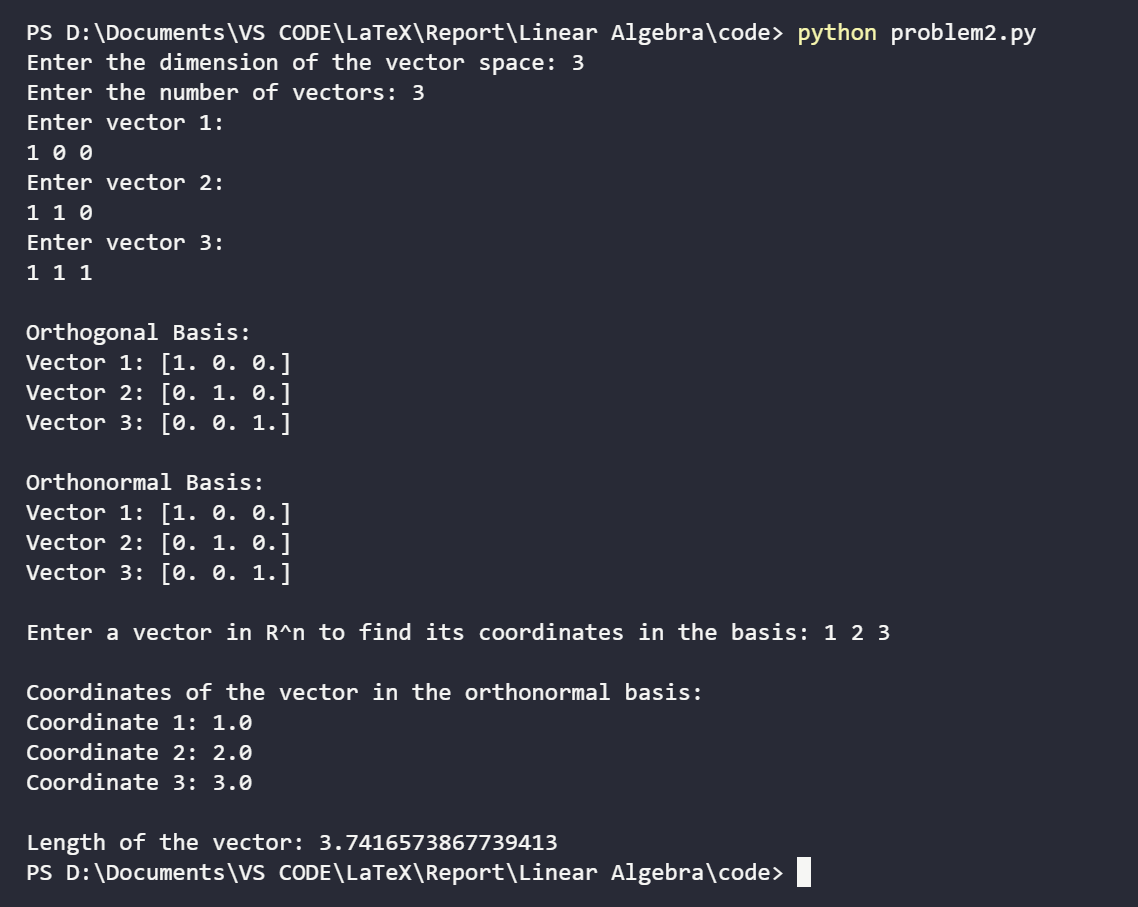
\includegraphics[width=16cm]{graphics/2.png}
    \caption{Console output of problem2.py}
\end{figure}
